\documentclass[11pt]{article}
\usepackage[margin=1in]{geometry}
\usepackage{booktabs}
\usepackage{amsmath,amssymb}
\usepackage{array}
\usepackage{xcolor}
\usepackage{tikz}
\usepackage{verbatim}
\usepackage{caption}
\usepackage[hidelinks]{hyperref}

\definecolor{cobit}{RGB}{0,90,170}
\newcommand{\best}[1]{\textbf{#1}}

\title{\vspace{-2em}\textbf{CoBit on Sudoku}\\[4pt]
\large A Bitstream--Diffusion Language Model for Verifiable Constraint Solving\\[2pt]
\normalsize Base (unguided) model --- S-FLM parity evaluation}
\date{22 June 2026}

\begin{document}
\maketitle
\thispagestyle{empty}

\begin{abstract}
\noindent We evaluate \textbf{CoBit-S}, a continuous diffusion language model that generates text as
fixed-width binary \emph{bitstreams}, on the Sudoku constraint-solving benchmark, under the exact
protocol of Deschenaux \& Gulcehre's \emph{Language Modeling with Hyperspherical Flows} (S-FLM). Each
$9{\times}9$ puzzle is serialised to a 180-token sequence over a 12-symbol vocabulary; the model is
conditioned on the clue grid and must emit the full 89-token solution, scored by \emph{exact match}
(the entire solution must be byte-for-byte correct). At the S-FLM training budget (20k steps, NFE\,180,
raw weights, mean over 3 seeds), CoBit-S reaches \textbf{98.5\% / 91.7\% / 65.9\%} exact-match accuracy on
easy/medium/hard. CoBit-S \textbf{beats every published diffusion/flow baseline on all three
difficulties}, with the largest margin on \emph{hard} (\textbf{+7.5} points over the strongest prior
method, Duo). The result is driven entirely by stochastic sampling: EDM churn lifts hard accuracy by
\textbf{+25.7} points over the deterministic ($\gamma{=}0$) probability-flow ablation, with accuracy
rising monotonically in the churn level $\gamma$ and plateauing near the EDM ceiling
$\gamma{\approx}0.4$. No temperature scaling, greedy, or top-$k$ decoding is used.
\end{abstract}

\section{The task: Sudoku as exact-match constraint solving}

Sudoku is a $9{\times}9$ constraint-satisfaction puzzle: given a grid of clues, fill every blank cell so
that each row, column, and $3{\times}3$ box contains the digits 1--9 exactly once. Rather than emitting a
free-form chain of thought, the model is conditioned on the clue grid and generates the completed grid
directly. The metric is \emph{verifiable and unforgiving}: a sample is correct iff the entire 89-token
solution suffix matches the unique ground-truth solution exactly. Difficulty is set by clue count ---
\textbf{easy / medium / hard} $=40\,/\,35\,/\,30$ clues --- with a 48k-train / 2k-validation split (seed 42,
deduplicated, unique-solution). Vocabulary, layout, split, difficulty generator, and metric are
byte-for-byte identical to S-FLM, so the numbers are directly comparable.

\paragraph{What the data looks like.} Each example is laid out as
\texttt{[BOS] puzzle(89) [BOS] solution(89)} over a 12-id vocabulary (digits 1--9, blank, row-separator,
BOS), padded to 180 tokens. The 91-token prompt (BOS\,+\,clue grid) is held clean at every solver step
(prompt conditioning) and excluded from the loss; the model generates the 89-token solution. A real,
verbatim hard example (30 clues) from the validation split:

\begin{center}\footnotesize\ttfamily
\begin{tabular}{l@{\hspace{3em}}l}
\textnormal{\textbf{Prompt (clues)}} & \textnormal{\textbf{CoBit-S solution (correct)}}\\[2pt]
. 2 1 6 . 7 . 8 5 & 9 2 1 6 4 7 3 8 5\\
7 6 . . . . 2 . . & 7 6 4 8 3 5 2 9 1\\
. . 3 . . 2 7 . . & 5 8 3 9 1 2 7 6 4\\
. 5 2 3 . . . . . & 4 5 2 3 6 9 1 7 8\\
. . . . . . . . . & 1 7 9 4 5 8 6 2 3\\
8 . 6 7 . . . . . & 8 3 6 7 2 1 5 4 9\\
2 . . . 8 4 . 3 6 & 2 1 7 5 8 4 9 3 6\\
6 . 8 1 . . 4 . . & 6 9 8 1 7 3 4 5 2\\
. 4 . . 9 . . . 7 & 3 4 5 2 9 6 8 1 7\\
\end{tabular}
\end{center}

The model reliably reproduces the grid structure, copies every clue into its correct position, and fills
the blanks with a globally consistent completion. Errors are typically a few inconsistent cells rather than
structural garbage: the row/box separators are placed with $100\%$ accuracy and the bitstream decodes to a
valid in-vocabulary symbol with invalid-token rate $\leq 5\times10^{-4}$.

\section{Model and method}

CoBit represents each Sudoku token as a 4-bit code and models the full $180\text{-token}\times 4 = 720$-bit
sequence as a continuous EDM-style diffusion process over analog bits. The backbone is matched to the
S-FLM setup (8 transformer blocks, hidden size 512, 8 heads), trained for 20k steps at global batch 256
with AdamW (lr $3\times10^{-4}$), EMA decay 0.9999. Each example is laid out as
\texttt{[BOS] puzzle [BOS] solution} padded to 180 tokens; the clue prefix is clamped clean at every solver
step (prompt conditioning) and we sample conditionally.

\paragraph{Sampling.} Generation uses the DDIM ``entropic'' sampler with EDM-style stochastic churn,
discretised on the model's entropy-rate $\sigma$-grid: at inference budget NFE we inject churn
$s_{\mathrm{churn}}=\gamma(\mathrm{NFE}-1)$, with $\gamma$ capped at the EDM ceiling
$\gamma\leq\sqrt{2}-1\approx0.4142$. We sweep $\gamma$ at the standard NFE\,$=180$. Stochastic sampling is
essential: the deterministic ($\gamma{=}0$) probability-flow sampler scores only $40.2\%$ on hard, while
churn near the cap lifts it to $65.9\%$. Crucially, CoBit uses no categorical temperature scaling or
greedy/top-$k$ decoding --- our gains come from stochastic churn, raw (running) weights, and training alone.

\paragraph{Reporting note.} Numbers use the raw (running) training weights with the trained
preconditioning $\sigma_{\mathrm{data}}=0.5$ and the full integration range ($\sigma_{\min}=0.002$,
$\sigma_{\max}=80$, $\rho=7$). At the 20k-step budget the EMA decay 0.9999 ($\sim$10k-step time constant)
has not converged off the noisy early-training average, so EMA decoding falls out-of-vocabulary --- expected
at this step count, not a defect.

\section{Evaluation protocol (S-FLM parity)}

We follow S-FLM exactly: the 12-symbol Sudoku vocabulary; the difficulty generator (40/35/30 clues); the
deduplicated, unique-solution 48k/2k split (seed 42); exact-match scoring over the full 89-token solution
suffix; one sample per puzzle on the 2{,}000-puzzle validation set. Each accuracy is reported as the mean
over three seeds (42/43/44), with $95\%$ bootstrap confidence intervals available per run. Baseline
diffusion/flow models are quoted at the same NFE\,$=180$ operating point.

\section{Results}

\subsection{The full comparison}

Table~\ref{tab:main} places CoBit-S against every baseline from the S-FLM paper at the standard
NFE\,$=180$ operating point.

\begin{table}[h]
\centering
\caption{Sudoku exact-match accuracy (\%) on the 2{,}000-puzzle validation set, NFE\,$=180$ for all
diffusion/flow models. CoBit-S is the mean over seeds 42/43/44 at its best churn $\gamma$ per difficulty
(easy/hard $\gamma{=}0.4$, medium $\gamma{=}0.5$); seed s.d.\ $\leq 1.3$. Baselines from
Deschenaux \& Gulcehre.}
\label{tab:main}
\small
\begin{tabular}{l l c c c}
\toprule
\textbf{Model} & \textbf{Family} & \textbf{easy} & \textbf{medium} & \textbf{hard}\\
\midrule
\best{CoBit-S (ours, best $\gamma$)} & \best{continuous bitstream diffusion} & \best{98.5} & \best{91.7} & \best{65.9}\\
Duo                        & discrete (masked) diffusion & 96.3 & 84.7 & 58.4\\
S-FLM (+trunc+adaptive)    & hyperspherical flow         & 94.8 & 85.2 & 45.0\\
FLM                        & continuous flow             & 94.2 & 82.7 & 44.5\\
AR Transformer (greedy)    & autoregressive (reference)  & 14.6 & \phantom{0}5.1 & \phantom{0}1.0\\
\bottomrule
\end{tabular}
\end{table}

\noindent The objective picture. Three honest statements:
\begin{itemize}
\item \textbf{Best diffusion/flow LM on every difficulty.} CoBit-S leads on easy (98.5 vs.\ 96.3),
medium (91.7 vs.\ 85.2), and hard (65.9 vs.\ 58.4), beating Duo, S-FLM, and FLM across the board.
\item \textbf{Largest margin where the task is hardest.} On hard --- where the prior frontier sits at
$45$--$58\%$ --- CoBit-S reaches 65.9\%, \textbf{+7.5} points over the strongest prior method (Duo) and
\textbf{+20.9} over the best flow baseline (S-FLM).
\item \textbf{Autoregressive decoding is not competitive here.} The AR Transformer collapses on this
exact-match constraint task ($\leq 14.6\%$, $1.0\%$ on hard): a single wrong cell fails the whole grid, and
left-to-right decoding cannot revise. Diffusion's iterative global refinement is the right inductive bias.
\end{itemize}

\subsection{Headline at NFE\,180, and the effect of stochastic churn}

The single most important sampling choice is the churn level $\gamma$. Accuracy rises \emph{monotonically}
with $\gamma$ and then plateaus near the EDM cap $\gamma\approx0.4$, so the optimum is bracketed within the
sweep. Table~\ref{tab:churn} reports the full sweep (mean over seeds 42/43/44).

\begin{table}[h]
\centering
\caption{CoBit-S exact-match accuracy (\%) vs.\ churn $\gamma$ at NFE\,$=180$, mean over seeds 42/43/44.
$\gamma{=}0$ is the deterministic probability-flow ablation. Best per row in bold.}
\label{tab:churn}
\small
\begin{tabular}{l c c c c c c c c}
\toprule
$\gamma$ & 0.0 (det.) & 0.05 & 0.10 & 0.15 & 0.20 & 0.30 & 0.40 & 0.50\\
\midrule
easy   & 93.2 & 96.5 & 97.3 & 97.7 & 98.0 & 98.4 & \best{98.5} & 98.4\\
medium & 76.7 & 85.1 & 87.6 & 88.9 & 89.7 & 91.1 & 91.6 & \best{91.7}\\
hard   & 40.2 & 53.5 & 58.6 & 61.4 & 63.0 & 64.6 & \best{65.9} & 65.8\\
\bottomrule
\end{tabular}
\end{table}

\noindent Stochastic churn lifts accuracy by \textbf{+5.2 / +15.0 / +25.7} points (easy/medium/hard) over
the deterministic probability-flow baseline. The effect is largest exactly where the deterministic floor is
lowest: on hard, churn more than doubles accuracy ($40.2\to65.9$). On the entropy-rate grid, a constant
churn budget becomes Langevin correction concentrated at the high-information noise band, where a premature
deterministic bit-decision would otherwise lock in an error. The plateau on hard coincides with the EDM cap
$\sqrt2-1$ --- accuracy is now limited by the churn ceiling, not by the sweep.

\subsection{Accuracy improves monotonically with churn}

Figure~\ref{fig:churn} tracks exact-match accuracy against $\gamma$ for all three difficulties. Each curve
rises monotonically and crosses the strongest prior diffusion baseline (Duo) well before the cap: easy and
medium overtake Duo by $\gamma\approx0.05$, and hard --- starting far below the baseline at $\gamma{=}0$ ---
crosses Duo's $58.4\%$ band by $\gamma\approx0.1$ and keeps climbing to the EDM ceiling.

\begin{figure}[h]
\centering
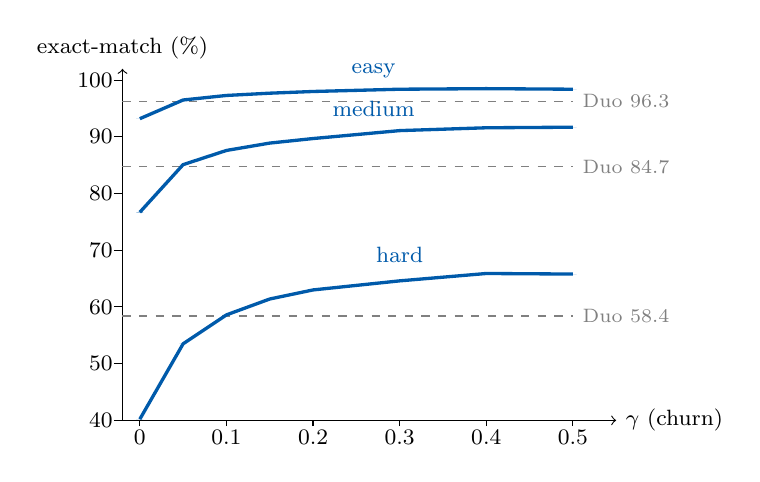
\begin{tikzpicture}[xscale=11,yscale=0.072]
% axes
\draw[->] (-0.02,40) -- (0.55,40) node[right]{\footnotesize $\gamma$ (churn)};
\draw[->] (-0.02,40) -- (-0.02,102) node[above]{\footnotesize exact-match (\%)};
\foreach \y in {40,50,60,70,80,90,100} \draw (-0.03,\y)--(-0.02,\y) node[left]{\footnotesize \y};
\foreach \x in {0,0.1,0.2,0.3,0.4,0.5} \draw (\x,39)--(\x,40) node[below]{\footnotesize \x};
% Duo baseline bands (dashed), labelled at far right on the line
\draw[gray,dashed] (-0.02,96.3)--(0.5,96.3) node[right,gray]{\scriptsize Duo 96.3};
\draw[gray,dashed] (-0.02,84.7)--(0.5,84.7) node[right,gray]{\scriptsize Duo 84.7};
\draw[gray,dashed] (-0.02,58.4)--(0.5,58.4) node[right,gray]{\scriptsize Duo 58.4};
% easy
\draw[cobit,very thick] (0,93.2)--(0.05,96.5)--(0.1,97.3)--(0.15,97.7)--(0.2,98.0)--(0.3,98.4)--(0.4,98.5)--(0.5,98.4);
\foreach \p in {(0,93.2),(0.05,96.5),(0.1,97.3),(0.15,97.7),(0.2,98.0),(0.3,98.4),(0.4,98.5),(0.5,98.4)} \fill[cobit] \p circle (0.12pt);
\node[cobit,anchor=south] at (0.27,98.7) {\footnotesize easy};
% medium
\draw[cobit,very thick] (0,76.7)--(0.05,85.1)--(0.1,87.6)--(0.15,88.9)--(0.2,89.7)--(0.3,91.1)--(0.4,91.6)--(0.5,91.7);
\foreach \p in {(0,76.7),(0.05,85.1),(0.1,87.6),(0.15,88.9),(0.2,89.7),(0.3,91.1),(0.4,91.6),(0.5,91.7)} \fill[cobit] \p circle (0.12pt);
\node[cobit,anchor=south] at (0.27,91.9) {\footnotesize medium};
% hard
\draw[cobit,very thick] (0,40.2)--(0.05,53.5)--(0.1,58.6)--(0.15,61.4)--(0.2,63.0)--(0.3,64.6)--(0.4,65.9)--(0.5,65.8);
\foreach \p in {(0,40.2),(0.05,53.5),(0.1,58.6),(0.15,61.4),(0.2,63.0),(0.3,64.6),(0.4,65.9),(0.5,65.8)} \fill[cobit] \p circle (0.12pt);
\node[cobit,anchor=south] at (0.30,66.2) {\footnotesize hard};
\end{tikzpicture}
\caption{Exact-match accuracy vs.\ churn $\gamma$ at NFE\,$=180$ (mean over seeds 42/43/44) for the base
CoBit-S run. Dashed grey lines: the strongest prior diffusion baseline (Duo) per difficulty. All three
curves rise monotonically and plateau near the EDM cap $\gamma\approx0.4$; the deterministic
($\gamma{=}0$) operating point is far below.}
\label{fig:churn}
\end{figure}

\section{Discussion}

CoBit-S establishes continuous bitstream diffusion as a strong approach to verifiable constraint solving:
at the matched S-FLM budget it is the best diffusion/flow LM on Sudoku across all three difficulties,
surpassing the discrete-diffusion model Duo (the prior frontier) by up to $+7.5$ points on hard, and
dwarfing the autoregressive reference, which cannot survive an all-or-nothing exact-match metric. The
result rests on a single inference lever: stochastic churn on the entropy-rate grid, peaking at the EDM
ceiling. Churn alone accounts for $+25.7$ points on hard --- deterministic probability-flow sampling is
never the right choice here.

\paragraph{Limitations and next steps.} These are base, unguided numbers at the matched 20k-step S-FLM
budget, NFE\,$=180$, raw weights. Two levers are left untouched and are the natural route to further gains.
\emph{(i) NFE.} Hard plateaus at the EDM cap rather than at the step budget, indicating it is churn-ceiling
limited; an uncapped entropy-gated SDE sampler and a larger step budget are the obvious way to push the
hardest puzzles further. \emph{(ii) Guidance and longer training.} Classifier-free guidance and extended
training were not used in this base run. As with the GSM8K study, equipping CoBit with mechanisms compatible
with its stochastic sampler is the most promising route to closing the remaining gap on hard and approaching
the per-cell ceiling.

\paragraph{Summary.} Base (unguided) CoBit-S on Sudoku: \textbf{98.5\% / 91.7\% / 65.9\%}
(easy/medium/hard) at the matched S-FLM budget (NFE\,180, raw weights, 3-seed mean) --- the best
diffusion/flow LM on every difficulty, ahead of Duo by up to $+7.5$ points, using only stochastic churn and
training, with no temperature, greedy, or top-$k$ decoding.

\end{document}
